\documentclass[11pt,a4paper]{scrarticle}
\usepackage[utf8]{inputenc}
\usepackage{cmap}
\usepackage[T2A]{fontenc}
\usepackage[russian]{babel}
\usepackage{amsmath,amssymb,amsthm,mathtools}
\usepackage{array}

\usepackage{indentfirst}
\usepackage{xcolor,graphicx, tikz, wrapfig}
\usepackage{longtable}
\usepackage{placeins}

\usepackage{minted}
\usemintedstyle{vs}

\usepackage[left=2cm,right=2cm,top=2cm,bottom=2cm,bindingoffset=0cm]{geometry}

\usepackage[unicode]{hyperref}
\definecolor{linkcolor}{HTML}{0000E6}
\definecolor{urlcolor}{HTML}{0000E6}
\definecolor{citecolor}{HTML}{0000E6}
\hypersetup{pdfpagemode=None,linktoc=page,citecolor=citecolor,linkcolor=linkcolor,urlcolor=urlcolor,colorlinks=true}

\theoremstyle{definition}
\newtheorem{subtask}{Пункт}

\DeclareMathOperator*{\argmax}{arg\,max}
\DeclareMathOperator*{\argmin}{arg\,min}
\newcommand{\floor}[1]{\left\lfloor #1 \right\rfloor}
\newcommand{\ceil}[1]{\left\lceil #1 \right\rceil}


\setlength{\parindent}{1cm}

\author{Клычков Максим Дмитриевич}

\begin{document}

\centerline{\textbf{\huge Алгоритмы и структуры данных-1}}
\centerline{\textbf{SET 3. Задача A2.}}
\begin{flushright}
	\emph{Осень 2024. Клычков М. Д.}
\end{flushright}

\begin{itemize}
	\item ID посылки по задаче \texttt{A1i}: \href{https://dsahse.contest.codeforces.com/group/NOflOR1Qt0/contest/565612/submission/292469913}{292469913}
	\item \href{https://github.com/maklybae/algorithms/tree/main/set03/a2}{Ссылка на репозиторий \texttt{GitHub}}
\end{itemize}

\subsection*{Внутренняя инфраструктура для экспериментального анализа}

Были реализованы классы \texttt{ArrayGenerator} и \texttt{SortTester} для организации удобного замера работы алгоритмов.

\begin{figure}[htp]
	\centering
	\inputminted[linenos,fontsize=\small]{cpp}{../analyze/generator.h}
	\caption{\texttt{ArrayGenerator Header File}}
	\label{code:generator-h}
\end{figure}
\FloatBarrier

\begin{figure}[htp]
	\centering
	\inputminted[linenos,fontsize=\small]{cpp}{../analyze/generator.cpp}
	\caption{\texttt{ArrayGenerator Cpp File}}
	\label{code:generator-cpp}
\end{figure}
\FloatBarrier

\begin{figure}[htp]
	\centering
	\inputminted[linenos,fontsize=\small]{cpp}{../analyze/tester.h}
	\caption{\texttt{SortTester Header File}}
	\label{code:tester-h}
\end{figure}
\FloatBarrier

\begin{figure}[htp]
	\centering
	\inputminted[linenos,fontsize=\small]{cpp}{../analyze/tester.cpp}
	\caption{\texttt{SortTester Cpp File}}
	\label{code:tester-cpp}
\end{figure}
\FloatBarrier

В функции \texttt{main()} происходит создание сразу трех объектов \texttt{SortTester} с разными \texttt{seed}. Каждый запуск происходит по три раза на каждом из тестеров, затем результаты усредняются.

В качестве значений \texttt{threshold} были выбраны числа $\{5, 10, 20, 50, 100, 200, 400\}$.

\emph{Некоторые замечания}: эта реализация не является оптимальной по крайней мере потому, что один и тот же код вызова сортировок повторятся для каждого алгоритма, однако было принято решение оставить такую реализацию, так как она уж точно не содержит никаких подводных камней, которые могут повлиять на временную оценку.

\subsection*{Анализ}

Для построения графиков использовался язык \texttt{Python}.

Для начала проанализируем маленькие значения \texttt{threshold}, а именно $\{5, 10, 20, 50\}$:

\begin{figure}[htp]
	\centering
	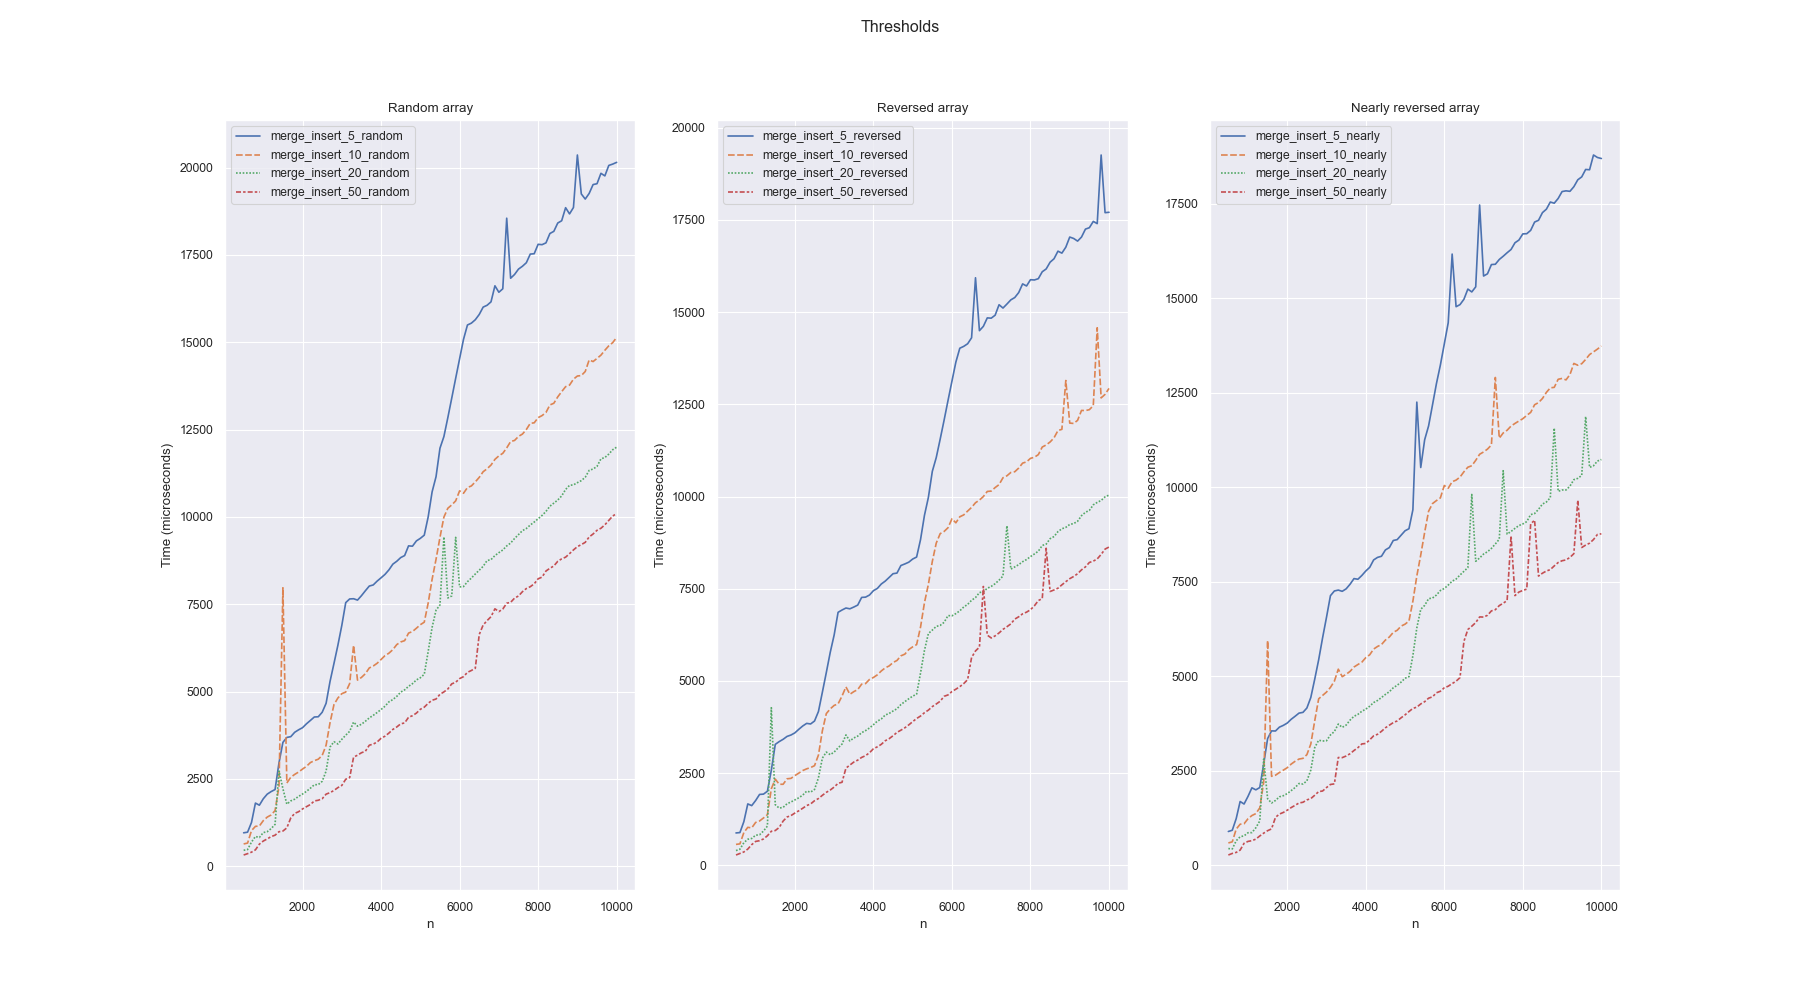
\includegraphics[width=\textwidth]{../static/thresholds_analysis_small_values.png}
	\caption{Малые значения \texttt{threshold}}
	\label{fig:thresholds-small}
\end{figure}
\FloatBarrier

Замечаем, что в любом случае (при любом типе сгенерированного массива) «побеждает» наибольшее здесь значение --- 50.

Сравним победителя с бОльшими значениями, а именно $\{100, 200, 400\}$:

\begin{figure}[htp]
	\centering
	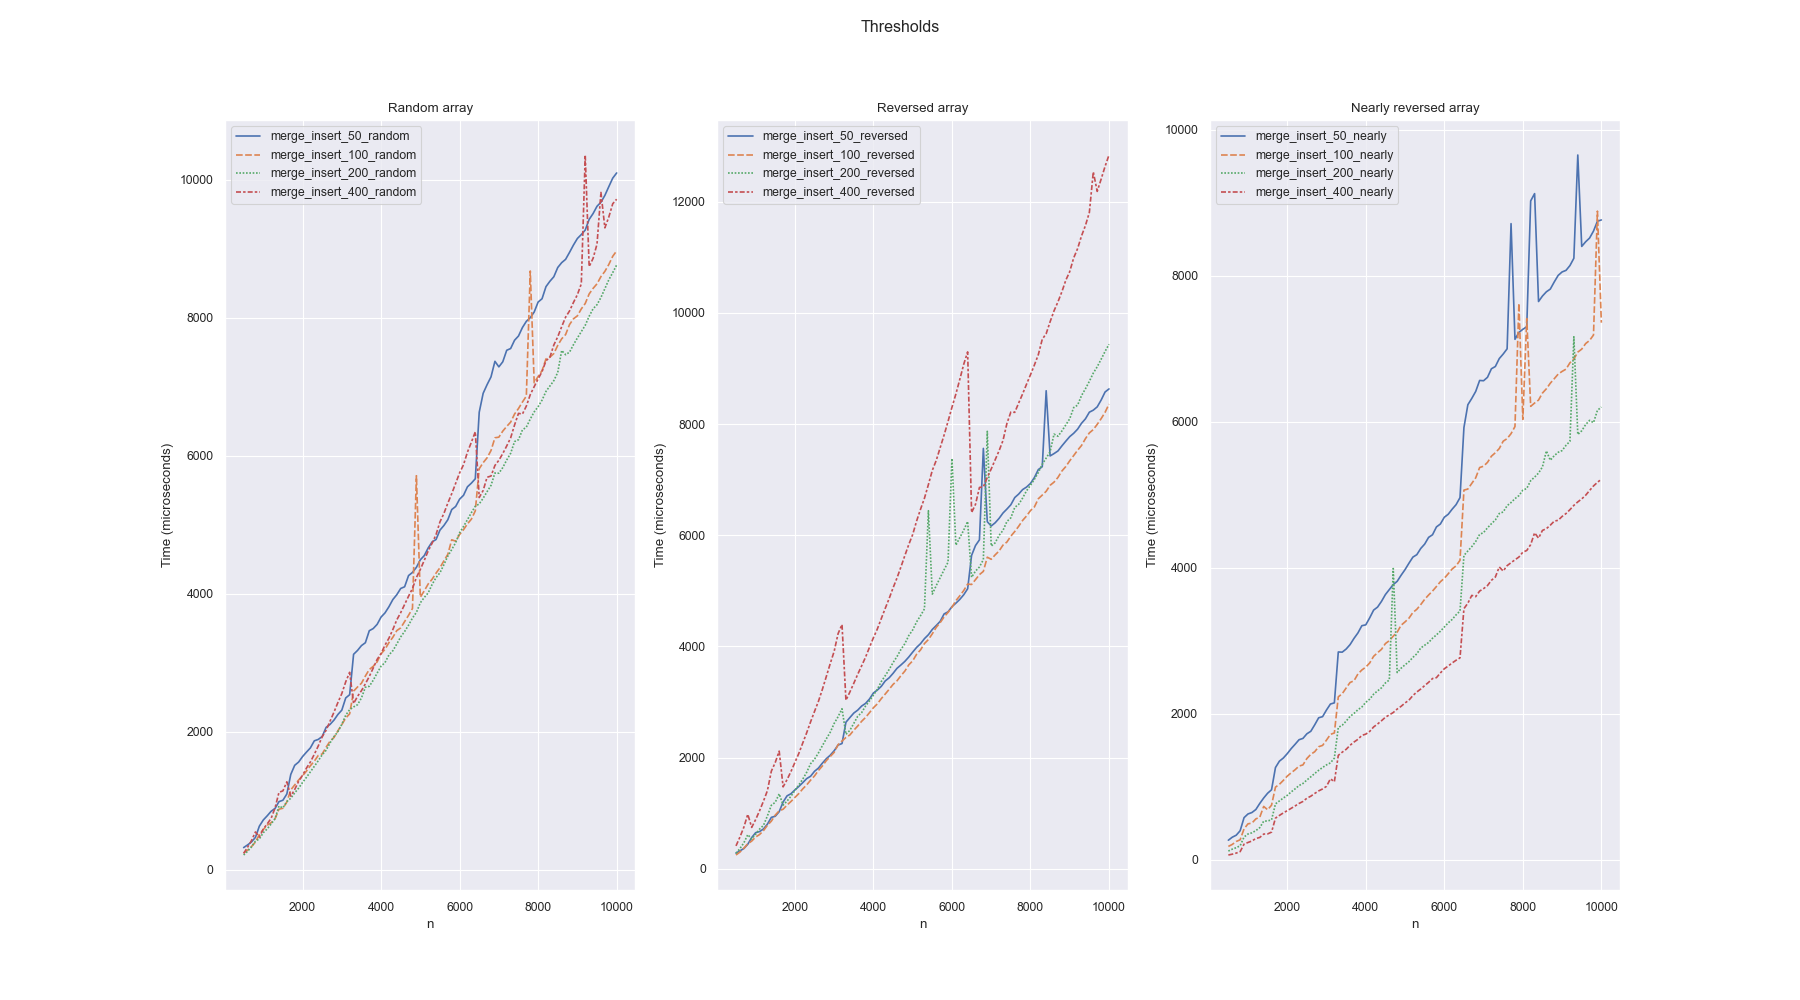
\includegraphics[width=\textwidth]{../static/thresholds_analysis_big_values.png}
	\caption{Большие значения \texttt{threshold}}
	\label{fig:thresholds-big}
\end{figure}
\FloatBarrier

Тут уже не такая однозначная ситуация. Наибольшее значение \texttt{threshold} имеет абсолютное преимущество только в одном случае --- практически отсортированный массив, и в то же время проигрывает всем другим значениям в отсортированных по убыванию массивах. Это объясняется тем, что сортировке вставками приходится работать на значительном количестве элементов, а, как известно, при отсортированном массиве \texttt{Insertion sort} линейна по времени, при обратно отсортированном --- квадрат.

Интересно увидеть это на другом графике:

\begin{figure}[htp]
	\centering
	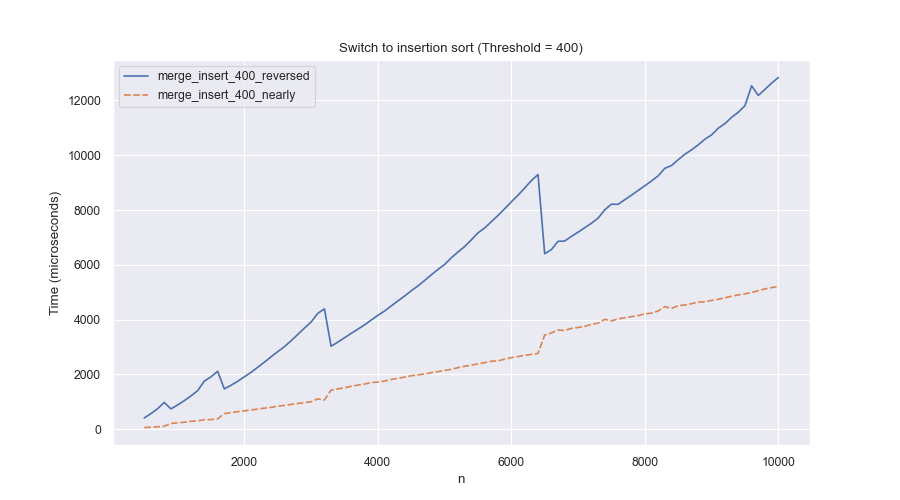
\includegraphics[width=0.5\textwidth]{../static/switch_to_insertion_sort.png}
	\caption{Переход на \texttt{Insertion Sort}}
	\label{fig:switch-insertion}
\end{figure}
\FloatBarrier

Четко виден момент, когда \texttt{Insertion Sort} работает на максимальном количестве элементов --- 400 (\emph{напомню} шаг 100), затем сразу резкий спуск --- на долю \texttt{Insertion Sort} выпадает меньшее количество элементов.

\emph{Вернемся к основной линии повествования}. Лучшие временные показатели на всех видах массивов показали значения \texttt{threshold} 100 и 200, поэтому далее будем рассматривать их.

\begin{figure}[htp]
	\centering
	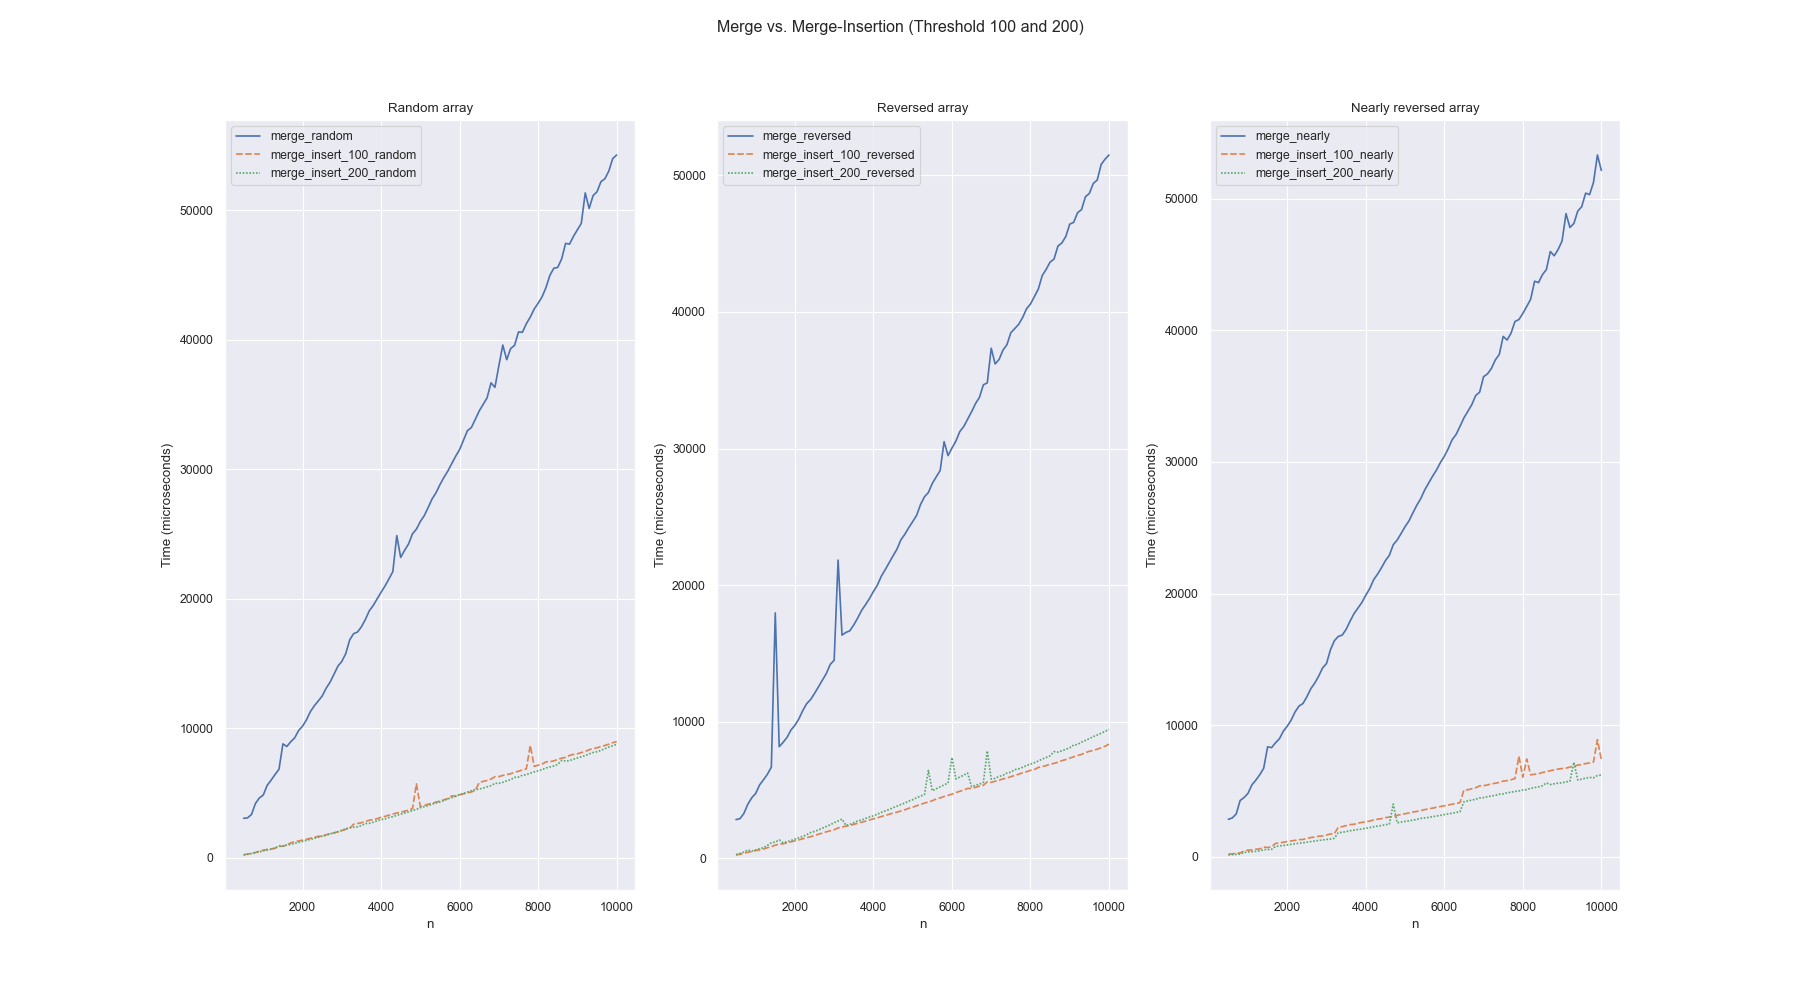
\includegraphics[width=\textwidth]{../static/merge_vs_merge_insertion.png}
	\caption{\texttt{Merge Sort} \emph{vs.} \texttt{Merge-Insertion Sort}}
	\label{fig:merge-vs-merge-ins}
\end{figure}
\FloatBarrier

Невооруженным глазом видно, что лидирует сортировка \texttt{Merge-Insertion Sort}, преимущество $\approx 5$ раз.

Единственный вопрос, оставшийся нерассмотренным, ---  сравнение сортировок по типам массивов.

\begin{figure}[htp]
	\centering
	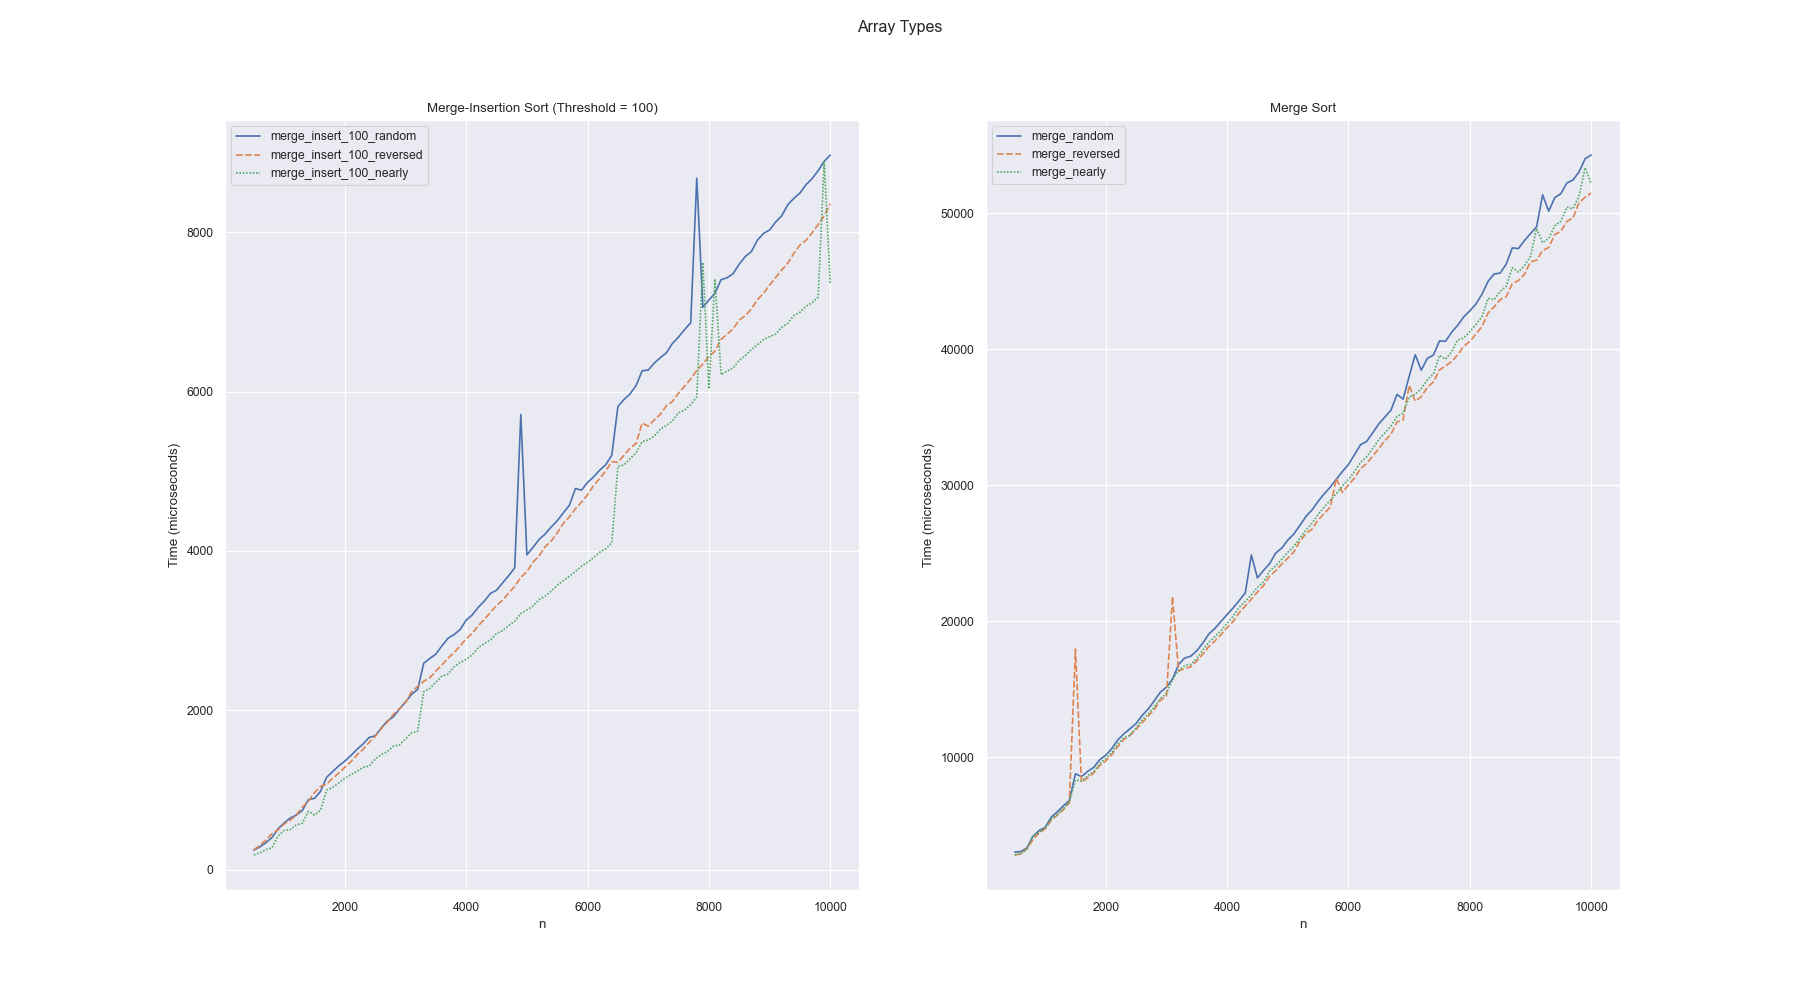
\includegraphics[width=0.85\textwidth]{../static/array_types.png}
	\caption{Сравнение типов массивов}
	\label{fig:merge-vs-merge-ins}
\end{figure}
\FloatBarrier

Как мы можем увидеть для \texttt{Merge Sort} совсем неважно, какой массив подается на вход --- время сортировки не изменится. Что же касается \texttt{Merge-Insertion Sort} для \texttt{threshold} равном 100, тут уже наблюдается разброс, но главным образом это связано с описанным выше поведением \texttt{Insertion Sort} на разных типах массивов.

\section*{Выводы}

Основные выводы по графикам были сделаны выше, тут же только отметим, что в любом случае при выборе между этими двумя сортировками стоит использовать вариант \texttt{Merge-Insertion Sort}. Также отмечу, что у этой \emph{комбинированной} сортировки сохраняется свойство \emph{устойчивости}, так как им обладают оба \emph{родителя} --- \texttt{Merge Sort} и \texttt{Insertion Sort}.

\end{document}

